%
%Не забыть:
%--------------------------------------
%Вставить колонтитулы, поменять название на титульнике



%--------------------------------------

\documentclass[a4paper, 12pt]{article} 

%--------------------------------------
%Russian-specific packages
%--------------------------------------
%\usepackage[warn]{mathtext}
\usepackage[T2A]{fontenc}
\usepackage[utf8]{inputenc}
\usepackage[english,russian]{babel}
\usepackage[intlimits]{amsmath}
\usepackage{esint}
%--------------------------------------
%Hyphenation rules
%--------------------------------------
\usepackage{hyphenat}
\hyphenation{ма-те-ма-ти-ка вос-ста-нав-ли-вать}
%--------------------------------------
%Packages
%--------------------------------------
\usepackage{amsmath}
\usepackage{amssymb}
\usepackage{amsfonts}
\usepackage{amsthm}
\usepackage{latexsym}
\usepackage{mathtools}
\usepackage{etoolbox}%Булевые операторы
\usepackage{extsizes}%Выставление произвольного шрифта в \documentclass
\usepackage{geometry}%Разметка листа
\usepackage{indentfirst}
\usepackage{wrapfig}%Создание обтекаемых текстом объектов
\usepackage{fancyhdr}%Создание колонтитулов
\usepackage{setspace}%Настройка интерлиньяжа
\usepackage{lastpage}%Вывод номера последней страницы в документе, \lastpage
\usepackage{soul}%Изменение параметров начертания
\usepackage{hyperref}%Две строчки с настройкой гиперссылок внутри получаеммого
\usepackage[usenames,dvipsnames,svgnames,table,rgb]{xcolor}% pdf-документа
\usepackage{multicol}%Позволяет писать текст в несколько колонок
\usepackage{cite}%Работа с библиографией
\usepackage{subfigure}% Человеческая вставка нескольких картинок
\usepackage{tikz}%Рисование рисунков
\usetikzlibrary{circuits} % подключаем библиотеки, содержащие
\usetikzlibrary{circuits.ee} % УГО для схем
\usetikzlibrary{circuits.ee.IEC}
\usetikzlibrary{arrows} % подключаем библиотеки со стрелками
\usetikzlibrary{patterns} % и со штриховкой
\usepackage{float}% Возможность ставить H в положениях картинки
% Для картинок Моти
\usepackage{misccorr}
\usepackage{lscape}
\usepackage{cmap}
\usepackage{bm}
\newtheorem{definition}{Опредление}



\usepackage{graphicx,xcolor}
\graphicspath{{Pictures/}}
\DeclareGraphicsExtensions{.pdf,.png,.jpg}

%----------------------------------------
%Список окружений
%----------------------------------------
\newenvironment {theor}[2]
{\smallskip \par \textbf{#1.} \textit{#2}  \par $\blacktriangleleft$}
{\flushright{$\blacktriangleright$} \medskip \par} %лемма/теорема с доказательством
\newenvironment {proofn}
{\par $\blacktriangleleft$}
{$\blacktriangleright$ \par} %доказательство
%----------------------------------------
%Список команд
%----------------------------------------
\newcommand{\grad}
{\mathop{\mathrm{grad}}\nolimits\,} %градиент

\newcommand{\diver}
{\mathop{\mathrm{div}}\nolimits\,} %дивергенция

\newcommand{\rot}
{\ensuremath{\mathrm{rot}}\,}

\newcommand{\Def}[1]
{\underline{\textbf{#1}}} %определение

\newcommand{\RN}[1]
{\MakeUppercase{\romannumeral #1}} %римские цифры

\newcommand {\theornp}[2]
{\textbf{#1.} \textit{ #2} \par} %Написание леммы/теоремы без доказательства

\newcommand{\qrq}
{\ensuremath{\quad \Rightarrow \quad}} %Человеческий знак следствия

\newcommand{\const}{\text{const}} % Написание const в формулах

\newcommand{\qlrq}
{\ensuremath{\quad \Leftrightarrow \quad}} %Человеческий знак равносильности

\renewcommand{\phi}{\varphi} %Нормальный знак фи

\renewcommand{\epsilon}{\varepsilon}

\newcommand{\me}
{\ensuremath{\mathbb{E}}}

\newcommand{\md}
{\ensuremath{\mathbb{D}}}



%\renewcommand{\vec}{\overline}




%----------------------------------------
%Разметка листа
%----------------------------------------
\geometry{top = 3cm}
\geometry{bottom = 2cm}
\geometry{left = 1.5cm}
\geometry{right = 1.5cm}
%----------------------------------------
%Колонтитулы
%----------------------------------------
\pagestyle{fancy}%Создание колонтитулов
\fancyhead{}
%\fancyfoot{}
\fancyhead[R]{\textsc{Интерферометр Майкельсона}}%Вставить колонтитул сюда
%----------------------------------------
%Интерлиньяж (расстояния между строчками)
%----------------------------------------
%\onehalfspacing -- интерлиньяж 1.5
%\doublespacing -- интерлиньяж 2
%----------------------------------------
%Настройка гиперссылок
%----------------------------------------
\hypersetup{				% Гиперссылки
	unicode=true,           % русские буквы в раздела PDF
	pdftitle={Заголовок},   % Заголовок
	pdfauthor={Автор},      % Автор
	pdfsubject={Тема},      % Тема
	pdfcreator={Создатель}, % Создатель
	pdfproducer={Производитель}, % Производитель
	pdfkeywords={keyword1} {key2} {key3}, % Ключевые слова
	colorlinks=false,       	% false: ссылки в рамках; true: цветные ссылки
	linkcolor=blue,          % внутренние ссылки
	citecolor=blue,        % на библиографию
	filecolor=magenta,      % на файлы
	urlcolor=blue           % на URL
}
%----------------------------------------
%Работа с библиографией 
%----------------------------------------
\renewcommand{\refname}{Список литературы}%Изменение названия списка литературы для article
%\renewcommand{\bibname}{Список литературы}%Изменение названия списка литературы для book и report
%----------------------------------------
\begin{document}
	\begin{titlepage}
		\begin{center}
			$$$$
			$$$$
			$$$$
			$$$$
			{\Large{НАЦИОНАЛЬНЫЙ ИССЛЕДОВАТЕЛЬСКИЙ УНИВЕРСИТЕТ}}\\
			\vspace{0.1cm}
			{\Large{ВЫСШАЯ ШКОЛА ЭКОНОМИКИ}}\\
			\vspace{0.25cm}
			{\large{Факультет физики}}\\
			\vspace{5.5cm}
			{\Huge\textbf{{Отчёт}}}\\%Общее название
			\vspace{1cm}
			{\LARGE{<<Интерферометр Майкельсона>>}}\\%Точное название
			\vspace{1cm}
			{\LARGE{Блуменау М. И.}}\\
			\vspace{2cm}
			\vfill
			
\includegraphics[width = 0.2\textwidth]{HSElogo}\\
			\vfill
			Москва\\
			2021
		\end{center}
	\end{titlepage}
	
	\tableofcontents
	\newpage
	\addcontentsline{toc}{section}{Введение}
	\section*{Введение}
	Целью данной работы являлось исследование работы интерферометра Майкельсона и различных его применений. Интерферометр Майкельсона -- двухлучевой интерферометр, изобретённый Альбертом Майкельсоном. Данный прибор позволил впервые измерить длину волны света. В опыте Майкельсона интерферометр был использован Майкельсоном и Морли для проверки гипотезы о светоносном эфире в 1887 году. 
	\addcontentsline{toc}{section}{Теоретическая справка}
	\section*{Теоретическая справка}
	\addcontentsline{toc}{subsection}{Минимумы и максимумы интерференции}
	\subsection*{Минимумы и максимумы интерференции}
	Рассмотрим интенсивность света, получаемую при интерференции от двух монохроматических источников с разностью фаз $\delta \phi$ :
	\begin{equation}
				I \propto ( \mathbf{E}^2_1 \cos(\mathbf{kr} - \omega t)|^2 )_t +
				( |\mathbf{E}^2_2 \cos(\mathbf{kr} - \omega t + \delta \phi)|^2)_t+ (|\mathbf{E}_1 \mathbf{E}_2\cos(\mathbf{kr} - \omega t)\cos(\mathbf{kr} - \omega t + \delta \phi)|)_t
	\end{equation}
	Допустим, интенсивность источников одинакова, тогда:
	\begin{equation}\label{int}
		I = 2 I_0 (1 + \cos{\delta\mathbf{\phi}})
	\end{equation}
	Исходя из полученного соотношения, зная, что $\delta \phi = \frac{2 \pi}{\lambda} \Delta$, где $\Delta$ - разность хода, а $\lambda$ -- длина волны, получаем условие максимумов и минимумов интерференционной картины:
	\begin{equation}\label{max}
		\Delta = m \lambda \text{ -- условие максимума}
	\end{equation}
	\begin{equation}\label{min}
		\Delta = (m + \frac{1}{2}) \lambda \text{ -- условие минимума}
	\end{equation}
	 Воспользумся знанием того, что сдвигая любое из зеркал на некоторое расстояние $\delta x$, разность хода составит $2\delta x$. В таком случае, из (\ref{max}) следует:
	\begin{equation}\label{deltax}
		2 \delta x = N \lambda,
	\end{equation}
	где $N$ -- число переходов максимум - минимум.
	\addcontentsline{toc}{subsection}{Интерферометр Майкельсона как спектральный прибор}
	\subsection*{Интерферометр Майкельсона как спектральный прибор}
	Чтобы рассмотреть использование интерферометра как спектрального прибора, имеет смысл вывести аналогичную (\ref{int}) формулу  для источников с отличающимися длинами волн:
	\begin{equation}
				I \propto( \mathbf{E}^2_1 \cos(\mathbf{k_1 r} - \omega t)|^2)_t +
				(|\mathbf{E}^2_2 \cos(\mathbf{k_2 r} - \omega t + \delta \phi)|^2)_t
				+( |\mathbf{E}_1 \mathbf{E}_2\cos(\mathbf{k_1r} - \omega t)\cos(\mathbf{k_2 r} - \omega t + \delta \phi)|)_t
	\end{equation}
	Данную формулу удобнее переписать в следующем виде (поскольку нас интересуют лишь изменяемые параметры, а интенсивности источников можно положить константными):
	\begin{equation}	
				I \propto (2 + \cos[(k_1 + k_2) \Delta / 2]) \cdot (\cos[(k_1 - k_2)\Delta/2])
	\end{equation}
	Из этого выражения, используя формулу для разности хода и (\ref{min}), получим условие минимума контрастности:
	\begin{equation}
		(\frac{\pi}{\lambda_1} - \frac{\pi}{\lambda_2}) \Delta = \pi (m + 1/2)
	\end{equation}
	Предполагая, что мы имеем дело с практически монохроматичным источником, перепишем:
	\begin{equation}\label{sp}
		\Delta = (m + 1/2) \frac{\lambda_0^2}{2\Delta \lambda}
	\end{equation}
	\addcontentsline{toc}{subsection}{Определение коэффициента преломления оргстекла}
	\subsection*{Определение коэффициента преломления оргстекла}
	Перейдём к теоретическому рассмотрению опыта с нахождением коэффициента преломления оргстекла. Воспользуемся предлагаемой в инструкции к интерферометру схемой:
	\begin{figure}[H]
		\centering
		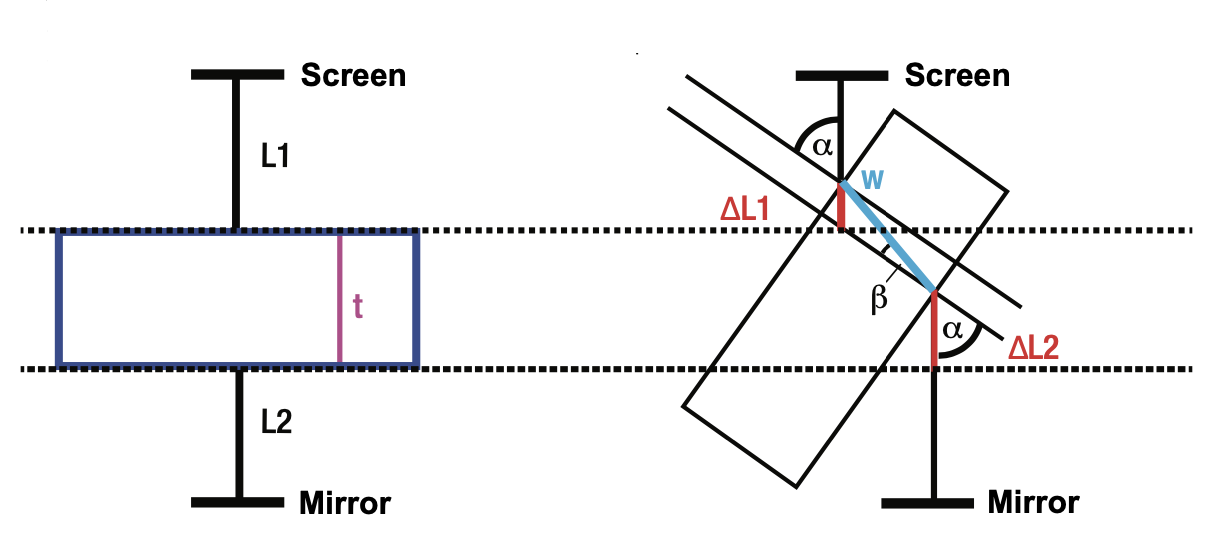
\includegraphics[width=0.85\linewidth]{sch1.png}
		\caption{Схематичное изображение пластинки перпедикулярно и под углом.}
		\label{fig:1}
	\end{figure}
	Полоожим $S1$ и $S2$ -- оптические пути для пластинки, перпендикулярной падающему свету и находящейся под углом $\alpha$ к лучу.
	\begin{equation}
		\begin{cases}
			S1= L1 + L2 + nt\\
			S2 = L1 + L2 + nw - \Delta L1 + \Delta L2
		\end{cases}
	\end{equation}
	где $L1, L2, w, t$ обозначены на Рис. \ref{fig:1}. Получим разность хода:
	\begin{equation}\label{delta}
		\Delta = n(w - t) - \Delta L1 + \Delta L2 = N \lambda
	\end{equation}
	Теперь выразим все неизвестные величины через ширину пластинки $t$ и углы:
	\begin{equation}\label{uset}
		\begin{cases}
			\Delta L1 = t \tan{\beta} \sin{\alpha}\\
			\Delta L2 = t (1 + \cos{\alpha}(\frac{\tan{\beta}}{\tan{\alpha}} - 1))\\
			w = \frac{t}{cos{\beta}}
		\end{cases}
	\end{equation}
	Из закона Снелла извезтно:
	\begin{equation}\label{snell}
		\cos{\beta} = \sqrt{1 - \frac{\sin^2{\alpha}}{n^2}}
	\end{equation}
	Из вышенаписанных (\ref{delta}), (\ref{uset}), (\ref{snell}), получим:
	\begin{equation}
		N \lambda = 2 t (\sqrt{n^2 - \sin^2{\alpha}} + 1 - \cos{\alpha} - n)
	\end{equation}
	Выразим коэффициент преломления:
	\begin{equation}\label{pn}
		n = \frac{(\frac{N \lambda}{2t} + \cos{\alpha} - 1)^2 + \sin^2{\alpha}}{2 (1 -\frac{N \lambda}{2t} - \cos{\alpha})}
	\end{equation}
	\addcontentsline{toc}{subsection}{Определение коэффициента теплового расширения}
	\subsection*{Определение коэффициента теплового расширения}
	При нагревании твёрдого тела, происходит его расширение. Это можно описать следующим уравнением:
	\begin{equation}
		\alpha=\frac{1}{L} \frac{\mathrm{d} L}{\mathrm{~d} T}
	\end{equation}
	Очевидным образом решаем данное дифференциальное уравнение и получаем:
	\begin{equation}
		L = L_0 \exp(\alpha \Delta T)
	\end{equation}
	Можно использовать линейное приближение данного закона:
	\begin{equation}
		\Delta L \approx L_0 \alpha \Delta T
	\end{equation}
	Воспользуемся уравнением (\ref{deltax}):
	\begin{equation}\label{hot}
		N = \frac{\alpha \Delta T L_0}{\lambda}
	\end{equation}
	\addcontentsline{toc}{section}{Оборудование и методы}
	\section*{Оборудование и методы}
	Оборудование: обучающий набор производства Thorlabs, включающий в себя оптический стол, светодиоды (красный и белый), зелёный лазер, делительный куб, зеркала, нагревательный элемент, вращательный стол, зажимы, линзу, пластинка, два куска оргстекла разной толщины.
	
	Для обработки результатов использовался язык программирования Python и совокупность пакетов Anaconda.
	Ссылка на исходный код:
	\newline \href{https://github.com/burunduk387/HSE-FF/tree/main/LabOptics/Фотонные\%20кристаллы}{https://github.com/burunduk387/HSE-FF/tree/main/LabOptics/Майкельсон}
	\begin{figure}[H]
	\centering
	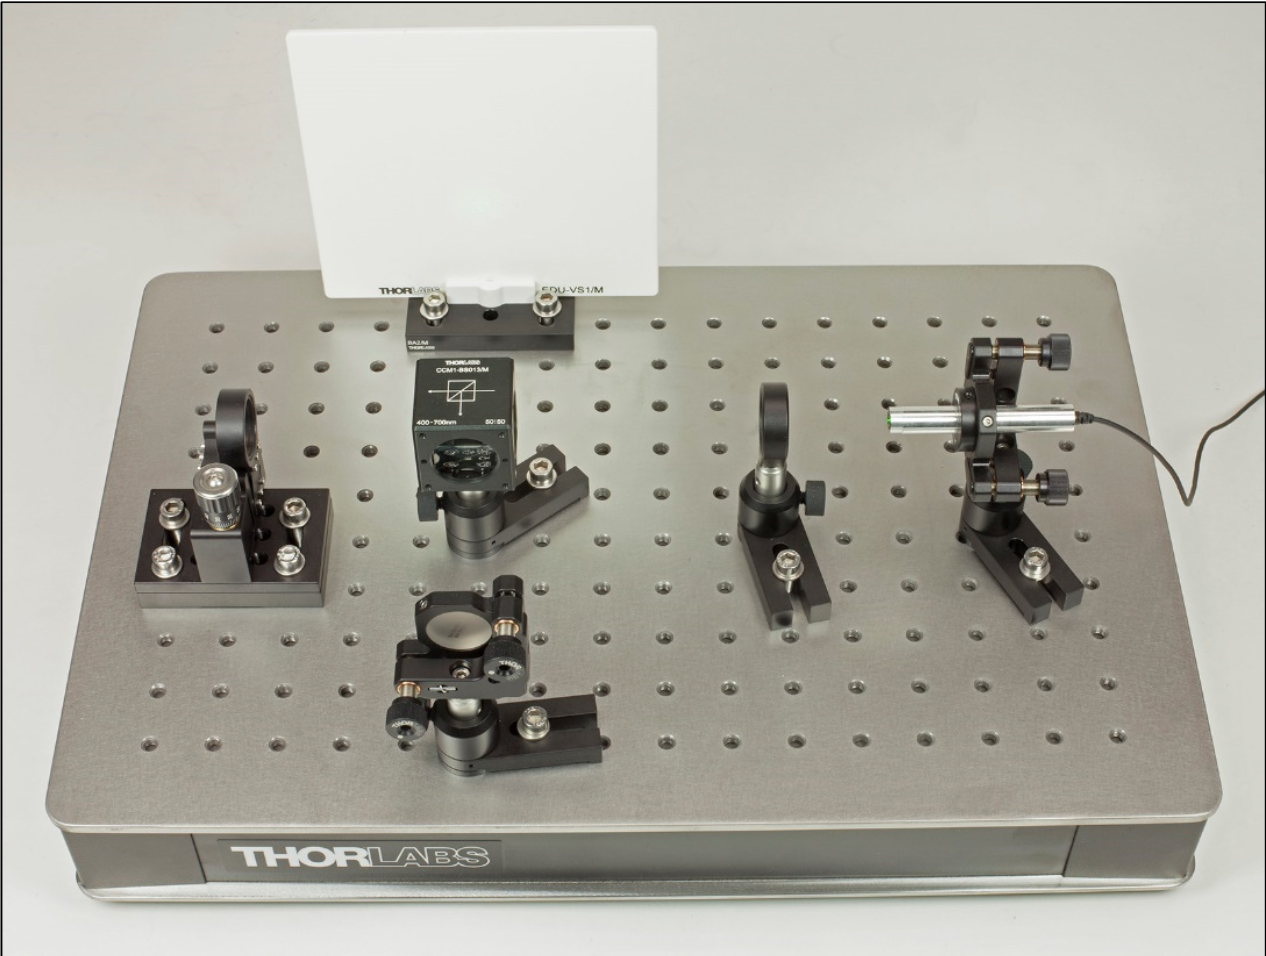
\includegraphics[width=0.75\linewidth]{Equip.png}
	\caption{Используемое оборудование.}
	\label{fig:2}
	\end{figure}
	\addcontentsline{toc}{section}{Эксперименты}
	\section*{Эксперименты}
	\addcontentsline{toc}{subsection}{Влияние длины плеча на интерференционную картину}
	\subsection*{Влияние длины плеча на интерференционную картину}
	Изменение расстояния между зеркалом на подвижном столе и делительным кубом приводило к видимому изменению интерфереционной картины: максимумы сменялись минимумами и наоборот, картина плыла.
	
	Данное поведение весьма предсказуемо. Из (\ref{int}) интенсивность зависит от разности фаз, которая линейно зависит от разности хода. Изменяя длину плеча, можно наблюдать на экране изменение интерференционной картины.
	\addcontentsline{toc}{subsection}{Опыт с зажигалкой}
	\subsection*{Опыт с зажигалкой}
	Нагрев воздух на некотором расстоянии от лазера (между кубом и лучом) было заметно похожее на предыдущий опыт поведение: максимумы сменялись минимумами и наоборот. 
	
	Рассуждения аналогичны предыдущему пункту, однако здесь причина кроется в изменении показателя преломления воздуха при изменении его температуры.
	\addcontentsline{toc}{subsection}{Наблюдение второго выхода интерферометра}
	\subsection*{Наблюдение второго выхода интерферометра}
	Часть света направлена в сторону лазера. Если поставить делительную пластину между кубом и лазером, можно пронаблюдать сразу две картины, что и показано на следующей фотографии.
	\begin{figure}[H]
		\centering
		\includegraphics[width=0.75\linewidth]{fig1.png}
		\caption{Фотография изображений, получаемых с двух выходов интерферометра.}
		\label{fig:3}
	\end{figure}
	Как можно заметить, максимуму одной картины соответствует минимум другой. Это очевидно из закона сохранения энергии.
	\addcontentsline{toc}{subsection}{Определение длины волны лазера}
	\subsection*{Определение длины волны лазера}
	Определим длину волны прилагаемого зелёного лазера. Используем для этого формулу (\ref{deltax}). Изменяя плечо интерферометра и считая количество переходов максимум-минимум, можно рассчитать длину волны.
	\begin{table}[H]
		\centering
		\caption{Таблица с полученными данными.}
		\begin{tabular}[t]{lcc}
			\hline
			Сдвиг зеркала, мкм&Количество переходов, шт.\\
			\hline
			5&19\\
			10&40\\
			15&57\\
			20&75\\
			25&90\\
			30&110\\
			\hline
		\end{tabular}
	\end{table}
	По этим данным можно построить график (приведён ниже) и подогнать его прямой, откуда с лёгкостью получаем длину волны: $\lambda = 531 \pm 17$ нм.
	\begin{figure}[H]
		\centering
		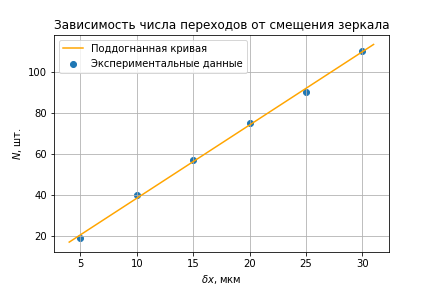
\includegraphics[width=0.85\linewidth]{maic1.png}
		\caption{График с полученными данными.}
		\label{fig:4}
	\end{figure}
	\addcontentsline{toc}{subsection}{Использование интерферометра как спектрометра}
	\subsection*{Использование интерферометра как спектрометра}
	Интерферометр можно использовать как спектральный прибор. Найдём такое положение зеркала, при котором будет наблюдаться минимальный контраст. Исходя из формулы (\ref{sp}), расстояние между положениями минимального контраста выражается через ширину спектра. После того, как найдём минимальный контраст, нужно найти следующее положение минимального контраста. Это положение находилось на расстоянии $850$ мкм, что соответствует ширине спектра $\Delta \lambda \approx 0.08$ нм. Данные в целом сходятся с данными для типичных лазеров данной ценовой категории. Точной спецификации лазера производитель, к сожалению, не предоставляет в открытом доступе.
	\addcontentsline{toc}{subsection}{Наблюдение интерференционной картины от светодидодов, когерентность}
	\subsection*{Наблюдение интерференционной картины от светодидодов, когерентность}
	Настроим с помощью лазерного модуля интерферометр так, что центральный максимум интерференционной картины как можно более крупный в размерах, а плечи интерферометра максимально близки друг к другу по длине. После этого заменим лазер на красный светодиод, вплотную поставив его к делительному кубу. Двигая одно из зеркал, заметим интерференционную картину. Повторив действия прошлого опыта находим длину когерентности красного светодиода, откуда легко вычисляется ширина спектра $\Delta \lambda \approx 14.62$ нм. То же самое повторим и с белым светодиодом. По очевидным причинам, здесь имеет смысл рассматривать только длину когерентности, она равна $L \approx 10$ мкм.
	 \addcontentsline{toc}{subsection}{Определение показателя преломления с помощью интерферометра}
	 \subsection*{Определение показателя преломления с помощью интерферометра}
	 Воспользуемся результатом (\ref{pn}). Для определения коэффициента преломления, необходимо знать толщину пластинки, угол ее отклонения и число переходов между максимумами и минимумами интерференционной картины. Толщины толстой и тонкой пластинок 12 и 7.5 мм, соответственно. Длина волны лазера была взята 532 нм. Результаты измерений представлены в таблице ниже:
	\begin{table}[H]
		\centering
		\caption{Таблица с полученными данными для толстой пластинки.}
		\begin{tabular}[t]{lcc}
			\hline
			Угол, градусы&Количество переходов, шт.\\
			\hline
			1&2\\
			1.5&5\\
			2&9\\
			2.5&13\\
			3&19\\
			3.5&25\\
			4&29\\
			\hline
		\end{tabular}
	\end{table}
	\begin{figure}[H]
		\centering
		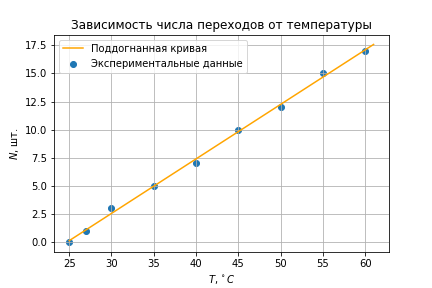
\includegraphics[width=0.85\linewidth]{maic2.png}
		\caption{График с полученными данными.}
		\label{fig:5}
	\end{figure}
	Получаем следующее значение коэффициента преломления:  $n = 1.43 \pm 0.04$.
	\begin{table}[H]
		\centering
		\caption{Таблица с полученными данными для тонкой пластинки.}
		\begin{tabular}[t]{lcc}
			\hline
			Угол, градусы&Количество переходов, шт.\\
			\hline
			2&7\\
			3&16\\
			4&25\\
			5&38\\
			6&49\\
			\hline
		\end{tabular}
	\end{table}
	Получаем следующее значение коэффициента преломления: $n = 1.59 \pm 0.09$.
	 \addcontentsline{toc}{subsection}{Измерение коэффициента теплового расширения}
	\subsection*{Измерение коэффициента теплового расширения}
	Воспользуемся собранным нагревательным элементом с прикреплённым к нему зеркалом. Подключим регулируемый блок питания и пустим ток. Элемент начнет нагреваться, удлиняться и двигать зеркало, что в свою очередь будет изменять интерференционную картину по закону (\ref{hot}). Температуру будем измерять термопарой. Результаты отображены в таблице ниже.
	\begin{table}[H]
		\centering
		\caption{Таблица с полученными данными при нагреве.}
		\begin{tabular}[t]{lcc}
			\hline
			Температура, градусы Цельсия&Количество переходов, шт.\\
			\hline
			25&0\\
			27&1\\
			30&3\\
			35&5\\
			40&7\\
			45&10\\
			50&12\\
			55&15\\
			60&17\\
			\hline
		\end{tabular}
	\end{table}
	Отсюда получаем значение параметра $alpha = 2.98 \cdot 10^{-5} \pm 0.22 \cdot 10^{-5} K^{-1}$ 
	\addcontentsline{toc}{section}{Вывод}
	\section*{Вывод}
	\begin{itemize}
			\item Изучены принципы работы интерферометра Майкельсона
			\item Найдена спектральная ширина лазера $\Delta \lambda \approx 0.08$ нм, красного светодиода $\Delta \lambda \approx 14.62$ нм, а также длина когерентности белого светодиода $L \approx 10$ мкм
			\item Найдены коэффициенты преломления нескольких пластинок из оргстекла: $n_{\text{тонк.}} = 1.59 \pm 0.09$, $n_{\text{толст.}} = 1.43 \pm 0.04$.
			\item Найден коэффициент теплового коэффициента расширения алюминия $alpha = 2.98 \cdot 10^{-5} \pm 0.22 \cdot 10^{-5} K^{-1}$ 
	\end{itemize}

	\addcontentsline{toc}{section}{Список литературы}
	\begin{thebibliography}{9}
		\bibitem{metod} 
		Thorlabs Michelson Interferometer.
		Методички к практикуму по оптике, 2021.
	\end{thebibliography}
\end{document}